
\section{Introduction}

For a long time, China has left behind a large number of historical documents, which have very important academic and artistic value. 
Therefore, in recent years, the study of historical documents has received widespread attention from researchers~\cite{jinic21,hde,obc306}. 

Different from other text recognition tasks, historical document recognition tasks face unique challenges like complexity and damage to the characters in historical documents, including stains, tears, and ink bleeding. 
In addition to the complexity of text recognition of historical documents, another major problem comes from the data itself. Specifically, history document recognition suffers from the long-tailed character occurrence distribution~\cite{obc306mk2}. 
The long-tailed distribution also affects other text recognition tasks like~\cite{fudanvi}, however, historical document recognition suffers a larger ``longtailness'' measured by the Gini Coefficient~\cite{tailsurvey}(See Figure~\ref{fig:moretailed}). 
Furthermore, novel characters can appear in the testing data~\cite{jinic21}, making it a hybrid of zero-shot and long-tail problems.

\begin{figure}[!t]
	\centering
	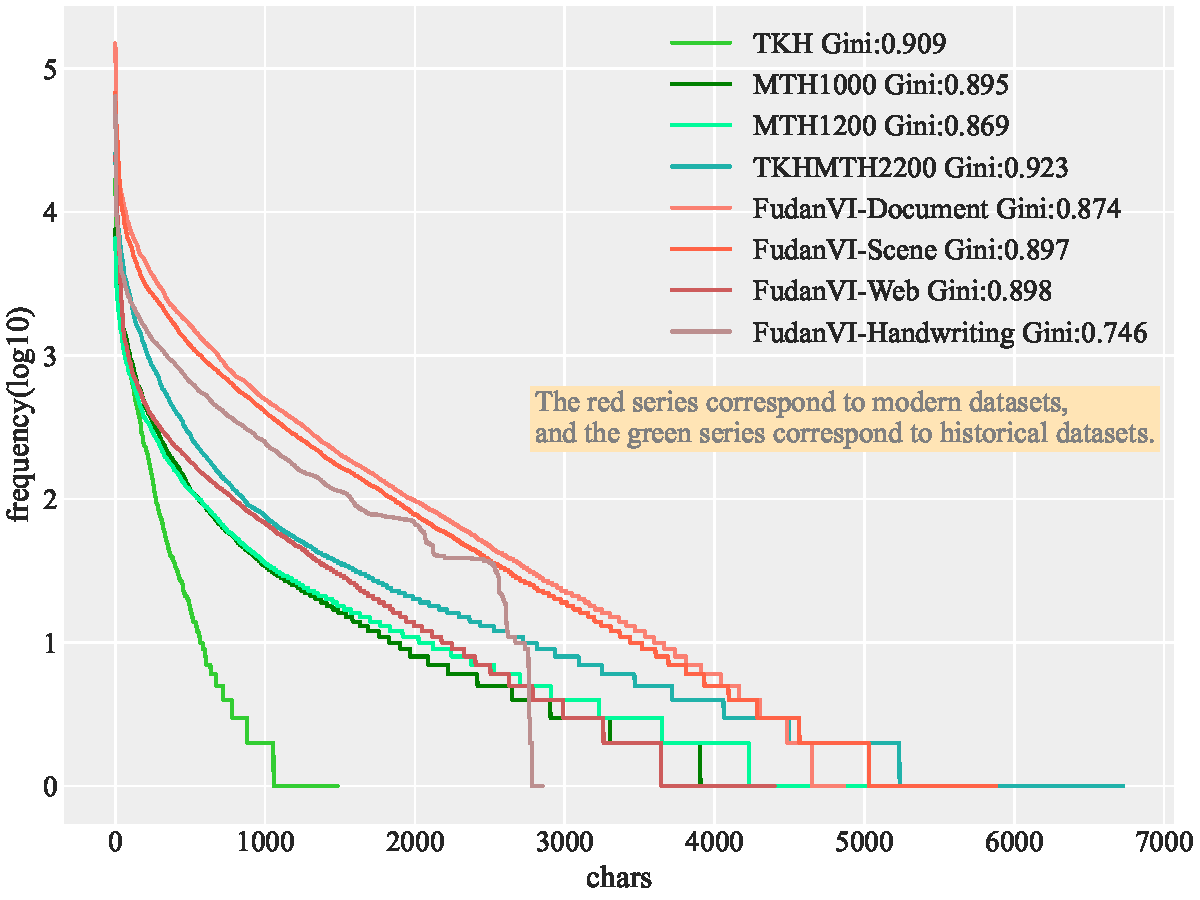
\includegraphics[width=\linewidth]{figures/database_long_tail.pdf}
	\caption
    {Comparison on Gini Coefficient~\cite{tailsurvey} between modern text recognition datasets~\cite{fudanvi} and historical text recognition datasets~\cite{tkhmth}.}
	\label{fig:moretailed}
\end{figure}

To address this challenge, existing methods propose to exploit the radical information of each character~\cite{denseran}, where individual radicals are often used in both head and tail (including unseen) classes, which are shown to generalize well in recognizing the novel characters~\cite{fewran,zhang20pr}.
On the other hand, Zhang et. al.~\cite{sanicdar23}  proved that exploiting the component information can improve the performance of tail classes.
However, such methods depend on radical-level annotations to train, yielding expensive annotation costs to deploy.

In this work, we propose to break free from the radical annotation by adopting a visual matching approach~\cite{vsdf}. 
To keep exploiting the similarity of character components, we propose implicitly emphasizing detail feature modeling.  
Specifically, we propose the spindle backbone network, which increases the number of parameters to shallow layers, which tends to extract character component features according to Howard et. al~\cite{mobile}. The network also reduces the parameters in deeper layers to keep the total parameter to keep a small vram footprint and high inference speed. 

The results indicate that the design effectively improves the model performance on tail classes. The approach also possesses decent recognition capability on novel classes, which can reduce the efforts needed for adapting the model for new excavations.
 
In addition, the approach also helps improve the head classes as well. 

In summary, the main contributions of this paper can be considered as follows:
\begin{enumerate}[noitemsep]
    \item We found that the similarity of character components can be leveraged to improve the performance of tails in long-tail distribution data.
    \item We implement a spindle network to extract character component features, exploiting the similarity between character components to improve the performance of tail classes.
    \item We conduct extensive experiments on three challenging Chinese ancient book datasets (TKH, MTH1000, and MTH1200) to validate the superiority of our proposed method. The results show that our approach achieves state-of-the-art performance in this field.
\end{enumerate}

% The longtailed distribution also affect other text recognition tasks like~\cite{fudanvi}, however historical document recogntion suffers a larger skewness~\cite{}(See Figure~\ref{fig:moretailed}). 

%Research areas include document typesetting, text detection, and text recognition. Text recognition is one of the core tasks in historical document visual tasks.
%In real life, we often encounter random variable distributions that exhibit broader characteristics than the standard positive land distribution, called long-tail distributions. 
%A typical feature of these distributions is that a small number of individuals make significant contributions, resulting in the minority class dominating the data set (called the head class), while the majority class contains only a few data samples (called the tail class). Long-tail distribution is very common in ancient text recognition. The important reasons are: 1) The long-tail characteristics of human language itself. 2) The number of ancient books is not large. The long-tail problem is one of the important challenges often encountered in historical document text recognition tasks.


%Document digitization systems protect printed paper documents from direct manipulation and facilitate consultation, exchange and remote access.

%Document digitization systems usually consist of two main stages: layout analysis and text recognition. The layout analysis stage involves dividing the document image into regions of interest, which is a prerequisite for subsequent text recognition.
%The main challenge of historical documents lies in their complex background and diverse layout situations. Text recognition methods can be divided into character-based methods and sequence-based methods. Character-based recognition methods typically involve locating individual characters, then identifying and grouping them into lines of text. Sequence-based methods, on the other hand, regress text lines and treat text recognition as a sequence labeling problem.

